\documentclass[pdftex,12pt,letter]{article}
\usepackage[margin=0.75in]{geometry}
\usepackage{verbatim}
\usepackage{graphicx}
\usepackage{xspace}
\usepackage{cite}
\usepackage{url}
\usepackage[pdftex,pdfpagelabels,bookmarks,hyperindex,hyperfigures]{hyperref}

\newcommand{\pd}{protoDUNE\xspace}
%\newcommand{\pdsp}{pD/SP\xspace}
\newcommand{\xrd}{XRootD\xspace}
\newcommand{\expname}{\textit{NP04}\xspace}

\title{The \pd-SP DQM data nomenclature and data access}
\date{\today}
\author{M. Potekhin}


\begin{document}
\maketitle

\begin{abstract}
\noindent  The Data Quality Monitoring (DQM) in the Single-Phase \pd experiment will be accomplished by running a few types
of jobs -- which can be organized in workflows -- in CERN Tier-0 under the management of the prompt processing system (p3s),
with prompt access to the raw data produced by the DAQ.
The resulting DQM data and visual products will be served to the users via a web interface. To make access to these results
optimal, a system of conventions and tags (akin to a rudimentary metadata) needs to be put in place. This
note describes a few ideas in this area.
\end{abstract}

%%%%%%%%%%%%%
\section{Overview}
\subsection{About this note}
This note is work in progress. Only a few select types of DQM jobs have been defined and developed at the time of writing
so we only cover those. More material will be added as it is developed.

\subsection{Glossary}
\begin{description}
\item [TPC (or LArTPC)] -- the Liquid Argon Time Projection Chamber
\item [PD] -- photon detector
\item [CRT] - cosmic ray tagger
\item [p3s] -- the \pd prompt processing system
\item [BI] -- beam instrumentation such as TOF and Cherenkov detectors
\item [F-FTS] -- the File Transfer Service developed at FNAL, and/or its instances
\item [EOS] -- disk-based distributed mass storage at CERN
\item [payload] -- the job that does the actual computation for DQM (as opposed to infrastructure tasks)
\end{description}

\section{Payloads}
\subsection{TPC}
\label{sec:tpc_payloads}


\subsection{PD}
TBD

\noindent Below is the summary of the principal data characteristics for \expname at the two ends of their estimated range:

%\begin{table}[tbh]
%\centering
%\begin{tabular}{l l}
%\hline
%\textbf{Metric} & \textbf{Value} \\
%\hline
%\hline
%trigger rate            & 25 -- 50 Hz \\  \hline
%peak data rate          & 1.5 -- 3.0 GB/s \\ \hline
%daily data volume       &  25 -- 50TB \\ \hline
%3-day buffer capacity   & 150 -- 300TB \\  \hline
%\hline
%\end{tabular}
%\caption{\label{tab:data_char}Expected \expname data characteristics.}
%\end{table}

\subsection{BI}
\label{sec:bi_payloads}




% \begin{figure}[tbh]
%   \centering
%   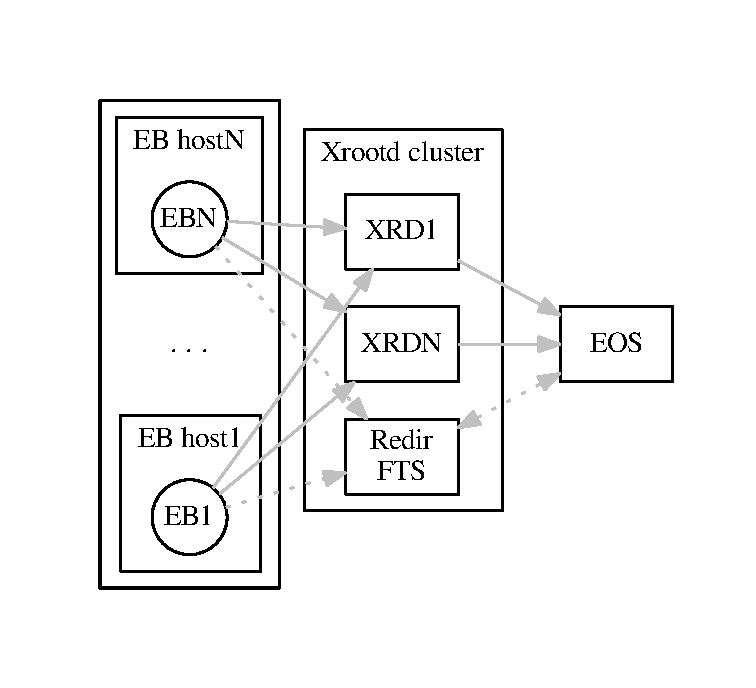
\includegraphics[width=0.5\textwidth]{../figures/doob-join.pdf}
%   \caption{Conceptual diagram of the Event Builders interfacing the XRootD cluster.}
%   \label{fig:doob-join}
% \end{figure}




\begin{thebibliography}{1}
\bibitem{docdb1086}
{DUNE DocDB 1086: \textit{ protoDUNE/SP data scenarios with full stream (spreadsheet)}}\\
\url{http://docs.dunescience.org:8080/cgi-bin/ShowDocument?docid=1086}

\bibitem{docdb186}
{DUNE DocDB 186: \textit{ ProtoDUNE Proposal}}\\
\url{http://docs.dunescience.org:8080/cgi-bin/ShowDocument?docid=186}


\bibitem{docdb1209}
{DUNE DocDB 1209: \textit{Basic Requirements for the protoDUNE Raw Data Mangement System}}\\
\url{http://docs.dunescience.org:8080/cgi-bin/ShowDocument?docid=1209}


\bibitem{docdb1212}
{DUNE DocDB 1212: \textit{Design of the Data Management System for the protoDUNE Experiment}}\\
\url{http://docs.dunescience.org:8080/cgi-bin/ShowDocument?docid=1212}



\bibitem{xrootd}
{XRootD, high performance, scalable fault tolerant access to data  repositories}.\\
  \url{http://xrootd.org/}.

\end{thebibliography}


\end{document}

%%% Local Variables:
%%% mode: latex
%%% TeX-master: t
%%% End:
